\def\pgfsysdriver{pgfsys-dvisvgm.def}
% flashcards-title: Qualitative matter budget for a growing organism
% flashcards-desc: A thick arrow enters an organism boundary, a thin arrow leaves it, and an upward arrow labeled stored matter increases appears inside.
\documentclass[tikz,border=6pt]{standalone}
\usetikzlibrary{arrows.meta,calc,fit,positioning,shapes.geometric}

\definecolor{fcink}{HTML}{17212B}
\definecolor{fcblue}{HTML}{1D5D8C}
\definecolor{fcgreen}{HTML}{2D6A4F}
\definecolor{fcorange}{HTML}{A44A1F}
\definecolor{fcpale}{HTML}{F4F7F9}
\definecolor{fcsoil}{HTML}{8B5E3C}

\tikzset{
  fc text/.style={font=\sffamily, text=fcink},
  fc panel/.style={draw=fcink, line width=0.9pt, rounded corners=5pt, fill=fcpale},
  fc node/.style={draw=fcink, line width=0.9pt, rounded corners=4pt, fill=white,
    minimum width=24mm, minimum height=10mm, align=center, font=\sffamily},
  fc arrow/.style={-{Stealth[length=3.2mm,width=2.4mm]}, line width=1.2pt,
    draw=fcblue, line cap=butt},
  fc boundary/.style={draw=fcorange, line width=1.4pt, dash pattern=on 5pt off 3pt,
    rounded corners=7pt},
  fc label/.style={font=\sffamily\bfseries, text=fcink},
  fc note/.style={font=\sffamily\small, text=fcink, align=center}
}

\begin{document}
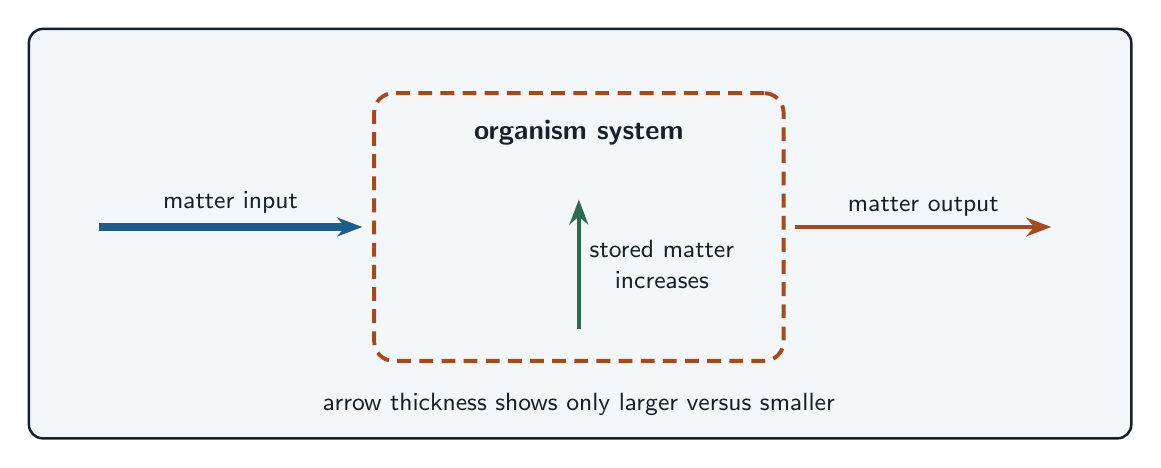
\begin{tikzpicture}[fc text, x=1cm, y=1cm]
  \node[fc panel, minimum width=140mm, minimum height=52mm, anchor=south west] at (0,0) {};
  \node[fc boundary, minimum width=52mm, minimum height=34mm] (org) at (7.0,2.7) {};
  \node[fc label] at (7.0,3.9) {organism system};
  \draw[-{Stealth[length=3.2mm,width=2.4mm]}, draw=fcblue, line width=3pt, line cap=butt]
    (0.9,2.7)--node[fc note, above] {matter input} (4.25,2.7);
  \draw[-{Stealth[length=3.2mm,width=2.4mm]}, draw=fcorange, line width=1.2pt, line cap=butt]
    (9.75,2.7)--node[fc note, above] {matter output} (13.0,2.7);
  \draw[fc arrow, draw=fcgreen] (7.0,1.4)--node[fc note, right] {stored matter\\increases} (7.0,3.05);
  \node[fc note] at (7.0,0.45) {arrow thickness shows only larger versus smaller};
\end{tikzpicture}
\end{document}
